\ylDisplay{Vooluring} % Ülesande nimi
{Koit Timpmann} % Autor
{lõppvoor} % Voor
{2018} % Aasta
{P 7} % Ülesande nr.
{3} % Raskustase
{
% Teema: Elektriõpetus

\ifStatement
Vooluringis on neli takistit väärtustega $R_1 = 2 \Omega$, $R_2 = 3 \Omega$, $R_3 = 6 \Omega$ ja $R_4 = 7 \Omega$. Punktide $C$ ja $D$ vahel on juhe, mille takistus on $0 \Omega$. Punktide $A$ ja $B$ vahele on rakendatud pinge suurusega $U = 18$ $V$. Kui suur on voolutugevus juhtmes $CD$?
\begin{center}
	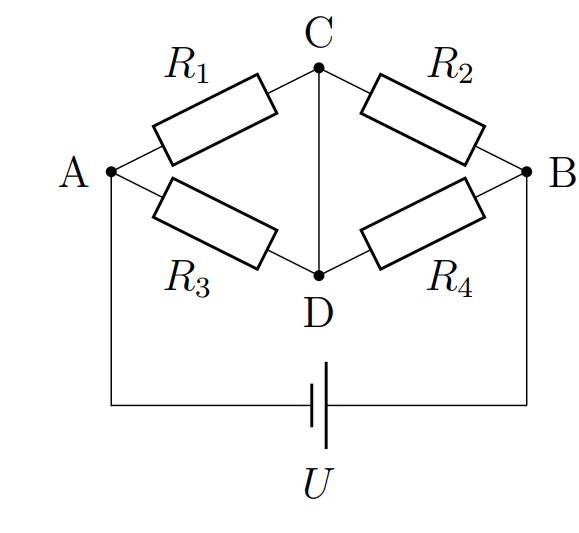
\includegraphics[width=0.5\linewidth]{2018-v3p-07-yl.png}
\end{center}
\fi

\ifHint
Kuna juhtmel $CD$ takistus puudub, võime vooluringi punktid $C$ ja $D$ lugeda samaks, mille korral on kaks rööbiti ühendatud takistit ühendatud teise rööpühendusega jadamisi.
\fi

\ifSolution
Kuna juhtmel $CD$ takistus puudub, võime vooluringi punktid $C$ ja $D$ lugeda samaks, mis punktis $C$. Sel juhul on vooluringis rööbiti ühendatud takistused $R_1$ ja $R_3$ ning takistused $R_2$ ja $R_4$ omavahel jadamisi ühendatud. 
Esimese rööpühenduse takistus:
\begin{center}
$R_{AC} = \frac{R_1 R_3}{R_1 + R_3} = 1,5$ $\Omega$.
\end{center}
Teise rööpühenduse takistus
\begin{center}
$R_{CB} = \frac{R_2 R_4}{R_2 + R_4} = 2,1$ $\Omega$.
\end{center}
Vooluringi kogutakistus $R = 3,6$ $\Omega$.
Arvutame vooluringis oleva voolutugevuse:
\begin{center}
$I = \frac{U}{R} = 5$ $A$
\end{center}
Vooluringi otstele rakendatud pinge jaguneb esimesele ja teisele rööpühendusele:
\begin{center}
$U_{AC} = I R_{AC} = 7,5$ $V$
\end{center}
\begin{center}
$U_{CB} = I R_{CB} = 10,5$ $V$.
\end{center}

Kuna takistid $R_1$ ja $R_3$ on rööbiti ühendatud, on pinge mõlema takisti otstel $7,5$ $V$. Takistite $R_2$ ja $R_4$ otstel on pinge $10,5$ $V$.
Ohmi seadusest saame, et voolutugevus takistis $R_1$ on
\begin{center}
$I_2 = \frac{U_2}{R_2} = 3,5$ $A$.
\end{center}
Seega punktist $C$ peab osa elektrivoolust liikuma mööda juhet $CD$ punkti $D$. Voolutugevus juhtmes $CD$ on
\begin{center}
$I_{CD} = I_1 - I_2 = 0,25$ $A$.
\end{center}
\fi
}